\section{Energy Profiling}

\setlength{\parskip}{5pt}

The paper ~\cite{DBLP:conf/intenv/Noureddine22} introduces two software tools for power monitoring on multiple platforms. The first tool, called PowerJoular, is written in the energy-efficient programming language Ada and enables runtime power monitoring of CPU and GPU in computers and servers, as well as CPU power consumption in Raspberry Pi devices. It utilizes Intel RAPL and NVIDIA's System Management Interface for PCs and servers, and its own empirical regression power models for Raspberry Pis. PowerJoular automatically detects the system configuration and provides power data accordingly, including monitoring of CPU power consumption of individual processes. It also offers a command-line interface and a systemd service for automatic monitoring during Linux boot, with data stored in a CSV file. JoularJX leverages PowerJoular, a previously introduced tool, to monitor power consumption at the method level in Java applications. It automatically initiates PowerJoular with appropriate parameters, writes power data to a CSV file, and provides live power consumption data for individual methods during runtime. JoularJX employs a statistical approach similar to Jalen, but with the added capability of monitoring power consumption at a finer-grained level. This tool offers developers and system tools the ability to track power consumption of individual methods in Java applications.\par


The study in JoularJX~\cite{DBLP:conf/intenv/Noureddine22} demonstrates the multi-platform capabilities of PowerJoular by measuring the energy consumption of three implementations of the Ray-casting algorithm on different devices. The experiments were conducted on a Dell laptop running Fedora Linux, a Raspberry Pi 3b+, and a Raspberry Pi 4B, each with different software stacks. The purpose was to showcase PowerJoular's ability to accurately monitor power consumption across diverse platforms and provide energy consumption data for various software implementations.\par

The findings in JoularJX~\cite{DBLP:conf/intenv/Noureddine22} showed that energy consumption of the Ray-casting algorithm varied between Python and C implementations on different platforms. PowerJoular enabled cross-platform comparisons, revealing that Python consumed more energy on the Intel-based computer, but less on the Raspberry Pi devices compared to C. This information can help software developers make informed decisions about choosing the appropriate implementation for specific platforms, such as using C on servers and Python on Raspberry Pi, based on energy consumption considerations.\par

In their study using JoularJX~\cite{DBLP:conf/intenv/Noureddine22}, the authors conducted experiments with a modified version of the Ray casting program to analyze the energy consumption of individual methods. They added print commands in each method and a loop in the main method for 50,000 iterations, and collected total energy consumption data for all methods, including those from the Java Development Kit (JDK) and program-specific methods. JoularJX's capability to provide real-time energy consumption data for each method during program execution allowed the authors 
to identify the methods that consumed the most energy. This information can be valuable for developers seeking to optimize their code for energy efficiency.\par

This in-depth analysis helped developers understand the energy hotspots of their programs. JoularJX introduced power monitoring of methods in real-time, allowing developers and automated tools to detect power variations in real-time and understand power draws in different scenarios. Overall, the study demonstrated that PowerJoular and JoularJX can be incorporated into integrated development environments (IDEs), testing frameworks, or used in pre-production servers to help developers understand power consumption in software and write power-efficient multi-platform software.\par


\section{Code Refactoring and Energy Efficiency}

\setlength{\parskip}{5pt}

 The paper ~\cite{DBLP:conf/esem/SahinPC14} focuses on the impact of code refactorings on energy usage in general software applications written in Java. The study examined nine Java applications with extensive JUnit test suites, representing both large and small projects from various domains. It focused on six selected refactorings that are commonly used and result in structural changes in the compiled bytecode. The considered six refactors are Convert Local Variable to Field, Extract Local Variable, Extract Method, Introduce Indirection,  Inline Method, Introduce Parameter Object. The applications were executed on JVM 7 and JVM 6, which have significant differences that can affect the impact of refactorings. The study utilizes specific tools for measuring energy consumption in Java applications. The primary tool employed is the Low Power Energy Aware Process (LEAP) node, which is an x86 platform with power sampling capabilities. It provides valuable data on the energy usage during the execution of the applications. The study followed a three-step procedure: Subject Creation involved applying the refactorings to create 197 refactored versions, ensuring coverage of executed code using the Clover tool. Data Collection involved measuring power usage, execution times, and dynamic execution counts using Apache Ant, synchronization information, and Clover coverage. Overall, the analysis showed that applying refactorings can have a significant impact on energy usage. The magnitude of the impact ranged from -7.50\% to 4.54\% in terms of percentage improvement in energy usage. However, refactorings are not consistent in their effects within and across applications, as well as within and across platforms. This emphasizes the need for considering energy efficiency during refactorings and highlights the contextual nature of their energy impact. Regarding the prediction of energy usage impact, the study explored the correlation between execution time and energy usage, finding a moderately strong positive correlation. However, it noted that execution time alone is not a reliable predictor of energy usage changes. Additionally, the study found no correlation between dynamic execution counts of refactored locations and energy usage impacts.
 
 
The ~\cite{DBLP:journals/ijebm/AcarAGG16} research paper addresses the need to understand and optimize the power consumption of software to develop sustainable and energy-efficient applications.  The proposed solution is the TEEC (Tool to Estimate Energy Consumption) model, which estimates power consumption by the CPU, memory, and disk during application runtime. TEEC enables developers to identify power-intensive code segments and optimize energy usage, resulting in the creation of energy-efficient software. The evaluation involves empirical experiments comparing the power consumption and execution times of optimized and unoptimized code. The study ~\cite{DBLP:journals/ijebm/AcarAGG16} emphasizes the significance of code optimization for energy efficiency, with the CPU's power consumption dominating over memory and disk. The results highlight the importance of developing optimized code to achieve green and efficient software. The TEEC tool considers the power consumption behavior of various components, and future work aims to integrate additional component power consumption for real-time guidance in building greener software. Existing tools and methodologies in related works lack accuracy or focus on specific components, making TEEC a valuable contribution to energy consumption estimation in software development.\par
 

In ~\cite{DBLP:journals/smr/FeitosaAAAN17} paper researchers empirically examine  the influences of Gang of Four (GoF) design patterns on energy consumption in object-oriented system design. It compares the energy usage of pattern-participating methods within GoF patterns to alternative solutions without patterns. The findings suggest potential negative effects of patterns on energy consumption, but also highlight cases where patterns may not adversely affect energy efficiency. The study~\cite{DBLP:journals/smr/FeitosaAAAN17} focuses on State, Strategy, and Template Method patterns and analyzes their energy consumption in open-source systems. The research follows an empirical approach, collecting data through usage scenarios and validating it using multiple measurements. The study ~\cite{DBLP:journals/smr/FeitosaAAAN17} concludes that alternative solutions are generally more energy-efficient, but patterns may be suitable for complex behaviors. Future work includes expanding the study~\cite{DBLP:journals/smr/FeitosaAAAN17} with more units and metrics and investigating other GoF patterns.\par

The paper ~\cite{DBLP:journals/tse/MoralesSKCA18} introduces EARMO, an energy-aware refactoring approach for mobile apps. It addresses the impact of coding practices and design choices on energy consumption by proposing a novel anti-pattern correction approach. EARMO considers energy consumption during the refactoring process and aims to reduce energy consumption in mobile apps, ultimately extending battery life. The study ~\cite{DBLP:journals/tse/MoralesSKCA18} evaluates EARMO on 20 Android apps and shows promising results, achieving a median removal of 84\% of anti-patterns and improving energy consumption by 48\%. The approach involves energy consumption estimation, code meta-model generation, and optimal refactoring sequences. It employs tactics such as anti-pattern identification, functionality redistribution, and search-based optimization. The paper ~\cite{DBLP:journals/tse/MoralesSKCA18} discusses related works on automated refactoring, Android anti-patterns, and energy consumption in mobile apps, highlighting the uniqueness of EARMO's approach. Future work includes expanding the detection of anti-patterns, applying EARMO to larger datasets, and conducting user studies to enhance its capabilities.\par


The paper ~\cite{DBLP:journals/infsof/PalombaNPZL19} explores the impact of code smells on the energy consumption of mobile applications, aiming to address the lack of knowledge in this area. Conducting a large-scale empirical investigation, the authors focus on 60 Android apps and nine method-level code smells. They utilize tools such as ADOCTOR for code smell detection and PETRA for energy estimation. The results highlight four specific energy smells that significantly affect energy consumption and emphasize the potential benefits of refactoring code smells. The paper ~\cite{DBLP:journals/infsof/PalombaNPZL19} underscores the importance of empirical evaluation in understanding the impact of code smells on energy efficiency in Android apps. The research mainly analyzes code at the method level, examining the influence of code smells on energy consumption within the application code. While the study does not delve into higher-level architectural aspects, it provides valuable insights into the correlation between code smells and energy consumption. The findings indicate a correlation between certain code smells and high energy consumption, but the impact of refactoring on reducing energy consumption was found to be insignificant. The paper ~\cite{DBLP:journals/infsof/PalombaNPZL19} concludes by emphasizing the significance of code quality-checkers, refactoring tools, and continued research to advance energy-efficient mobile app development. The related literature explores traditional code smells and their effects on program quality, detection, and refactoring, while limited empirical assessment exists for Android-specific code smells. The paper ~\cite{DBLP:journals/infsof/PalombaNPZL19} contributes to the field by analyzing a wider variety of code smells at the method level, providing valuable insights into energy efficiency in mobile apps.\par

\begin{table}[h]
\begin{adjustbox}{center}
\footnotesize
\begin{tabular}{|p{3cm}|p{4cm}|p{4.5cm}|p{2cm}|p{1.5cm}|}
  \hline
  \textbf{Reference} & \textbf{Code refactoring} & \textbf{Experiment/Benchmarking} & \textbf{Tool for EC} & \textbf{Results} \\
  \hline
  \cite{DBLP:conf/esem/SahinPC14} & 
  Convert Local Variable to Field, Extract Local Variable, Extract Method, Introduce Indirection, Inline Method, Introduce Parameter Object & 
  9 Java Applications (e.g., cMath, cCollections, ...) & 
  Low Power Energy Aware Process (LEAP) &
  -7.50\% to 4.54\% \\
  \hline
  \cite{DBLP:journals/tse/MoralesSKCA18} & 
  \textbf{Android code smells (3)}: Binding resources too early class, Private getter and setters, HashMap usage. \textbf{OO code smells (5)}: Lazy class, Blob (God class), Long-parameter list, Refused bequest, Speculative Generality & 
  \textbf{Phase 1:} Empirical Study to understand in which extent 8 code refactorings help to save energy. \textbf{Phase 2:} EARMO is developed to select optimal series of code refactoring.  The energy consumed by the version of code is inferred from Phase 1. & 
  Not reported. &
  EARMO is able to save 29 minutes of battery.\\
  \hline
  \cite{DBLP:journals/infsof/PalombaNPZL19} & 
  \textbf{Android-specific code smells (9)}: Data Transmission Without Compression, Durable Wakelock, Inefficient Data Structure, Inefficient SQL Query, Inefficient Data Format And Parser, Internal Setter, Leaking Thread,  Member-Ignoring Method, Slow Loop & 
  60 Android Java apps (categories ex. games, productivity, social, etc) & 
  PETRA (Power Estimation Tool for Android) & 
  Four code smell types increase method energy consumption by up to 87 times. \\
  \hline
\end{tabular} 
\end{adjustbox}
\caption{Comparison of approaches}
\label{tab:result}
\end{table}

%\vspace{1em}

\section{Genetic Improvement (GI)}

\setlength{\parskip}{5pt}
Genetic Improvement (GI) is a field of research that uses automated search to find improved versions of existing software~\cite{DBLP:conf/gecco/BrownleePABWW19}~\cite{DBLP:journals/tec/PetkeHHLWW18}. It can improve both functional properties of software, such as bug repair, and non-functional properties, such as execution time, energy consumption, or source code size~\cite{DBLP:conf/gecco/ZuoBP22}. Researchers have already shown that GI can improve human-written code, ranging from program repair to optimizing run-time, from reducing energy consumption to the transplantation of new functionality~\cite{DBLP:conf/gecco/BrownleePABWW19}.\par

GI uses optimization and machine learning techniques, particularly search-based software engineering techniques such as genetic programming to improve existing software. The improved program need not behave identically to the original. For example, automatic bug fixing improves program code by reducing or eliminating buggy behavior. In other cases, the improved software should behave identically to the old version but is better because it runs faster, uses less memory, uses less energy or runs on a different type of computer.\par

GI can be used with multi-objective optimization to consider improving software along multiple dimensions or to consider trade-offs between several objectives, such as asking GI to evolve programs that trade speed against the quality of answers they give. Of course, it may be possible to find programs that are both faster and give better answers. Mostly Genetic Improvement makes typically small changes or edits (also known as mutations) to the program's source code but sometimes the mutations are made to assembly code, byte code or binary machine code.\par

In theory, GI can be applied to any software. However, its effectiveness depends on many factors such as the quality of the test suite and the complexity of the software. It is an active area of research and new techniques and tools are being developed to make GI more effective and applicable to a wider range of software systems.\par

\subsection{The Gin toolbox}

\setlength{\parskip}{5pt}
Gin is a genetic improvement (GI) tool that aims to facilitate experimentation and research in the field of software development. It provides an extensible and modifiable toolbox for GI experimentation, specifically targeting the Java ecosystem. By automating the transformation, building, and testing of Java projects, Gin supports various aspects of software improvement, including program repair, runtime optimization, energy consumption reduction, and the addition of new functionality. The tool incorporates features such as automated test generation and source code profiling, which are essential for non-functional improvement. Gin's design focuses on scalability, allowing it to handle large-scale systems and integrate with popular Java build systems like Maven and Gradle. It supports multiple representations of code, providing flexibility for researchers to define custom mutation operators and transformation strategies. Additionally, Gin introduces innovative features for non-functional improvement, including built-in profiling and automated test case generation.\par

\begin{figure}[h]
  \centering
  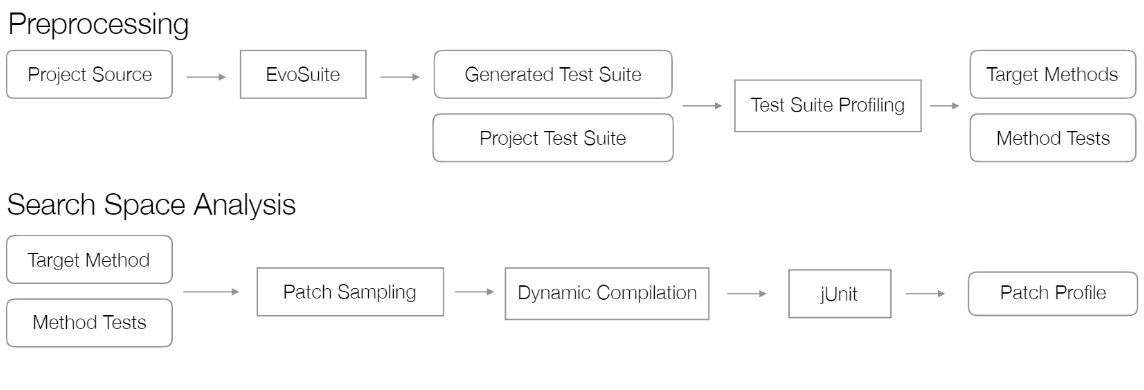
\includegraphics[width=1.0\textwidth]{img/Gin_Pipelines.png}
  \caption{Gin Pipelines~\cite{DBLP:conf/gecco/BrownleePABWW19}}
  \label{fig:GinPipelines}
\end{figure}


As shown in Figure \ref{fig:GinPipelines}, Gin provides two example pipelines for Preprocessing and Search Space Analysis.\par

\textbf{Preprocessing}: Gin can preprocess a project and find the methods that are most likely to benefit from genetic improvement (GI). This is done by using the gin.util.Profiler class, which measures the execution time of each method in the project and ranks them by their contribution to the overall performance. The methods with the highest execution time are called 'hot methods' and are output as suitable targets for improvement by GI.\par

\textbf{Search Space Analysis}: Gin can also help to analyze the search space of possible program edits that can be applied by GI. The toolkit provides several tools that can sample and enumerate different types of edits, such as statement deletion, insertion, or replacement. These tools can be easily extended or reused to add new edit types. Gin will test each sampled or enumerated edit by applying it to the original code and running a test suite against the modified code. Gin will record various information about each edit, such as its validity (whether it preserves the functionality of the original code), its compilation result, its test output (whether it passes or fails the test suite), its run time (how long it takes to execute the test suite), and its error details (if any). Gin can use any test suite that is in JUnit format, which is a widely used testing framework for Java. Gin can also capture more detailed test output than just pass or fail, such as the difference between the expected and actual output. This allows Gin to support more fine-grained fitness functions that can measure the quality of each edit more accurately.\par


\begin{figure}[h]
  \centering
  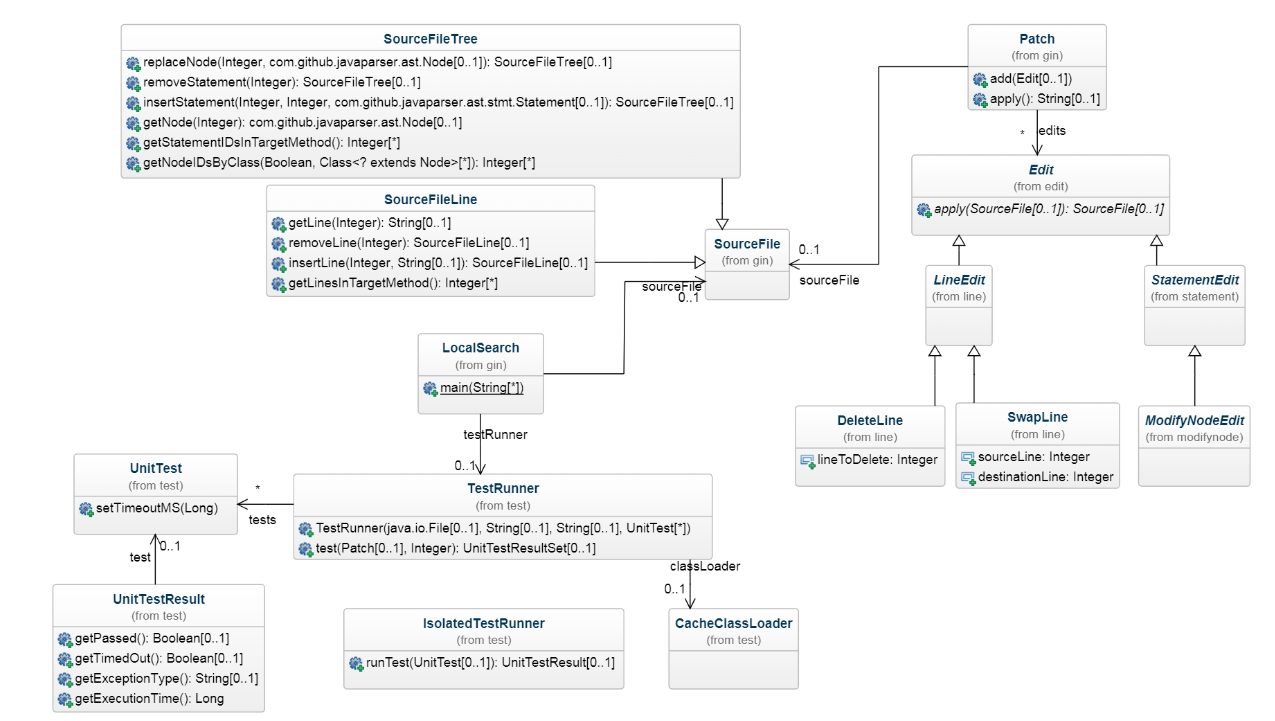
\includegraphics[width=1.0\textwidth]{img/Gin_Core_Classes.png}
  \caption{Gin Core Classes.~\cite{DBLP:conf/gecco/BrownleePABWW19}}
  \label{fig:Gin_Core_Classes}
\end{figure}



The Gin toolkit encompasses a collection of classes designed to facilitate genetic improvement research by offering a framework for manipulating source code, executing tests, and analyzing outcomes. At the core of this toolkit lies the SourceFile class, an immutable representation of the original source code, equipped with various methods for modifying the codebase, accessing language constructs, and generating modified Java source code.\par

Derived from the SourceFile class, the SourceFileTree subclass focuses on edits to the Abstract Syntax Tree (AST) of the source code. It assigns unique identifiers to each node within the AST, enabling efficient resolution of patches that entail multiple edits to the same location. In a similar vein, the SourceFileLine subclass directs its attention to line-level edits, also employing unique IDs for each line to simplify edit application.\par

A crucial component within Gin is the Patch class, which serves as a container for a series of edits, encapsulating the desired changes to be applied to the source code. The Edit class, serving as the base class for different types of edits, represents the application of a specific operator to the target source code. Subclasses of Edit, including LineEdit and StatementEdit, offer a range of operations for manipulating lines of code and modifying statements, respectively. The granularity of these edits provides fine-grained control over the code transformations.\par

To explore the search space of software transformations, the LocalSearch class employs a combination of sampling and searching techniques. It navigates through possible modifications to improve the code, ultimately enhancing its quality and performance. Meanwhile, the TestRunner class utilizes the JUnit framework to execute unit tests, offering insights into the outcomes, execution time, and encountered errors of the modified code.\par

The UnitTest class represents an individual unit test and is employed by the TestRunner to evaluate the test outcomes. Storing the result of a unit test, including pass/fail status, expected and actual results, and error details, the UnitTestResult class aids in analyzing the impact of code modifications on test behavior.\par

For focused testing of individual edits or patches, the IsolatedTestRunner subclass of TestRunner conducts tests in isolation. Finally, the CatcheClassLoader class, a custom ClassLoader, loads the modified class during test execution, overlaying the existing class hierarchy and facilitating the loading of the modified class by JUnit.\par

Collectively, these classes and their interplay within the Gin toolkit provide researchers with a powerful foundation for genetic improvement studies. The toolkit simplifies the process of editing source code, conducting tests, and evaluating the effects of modifications, thereby enabling more efficient and effective research in this domain.\par
